\documentclass{beamer}

\usepackage[brazilian]{babel}
\usepackage[utf8]{inputenc}
\usepackage[T1]{fontenc}
\usepackage{xcolor}
\usepackage{listings}
\usepackage{color}
\usepackage{courier}
\usepackage{tikz}
\usepackage{verbatim}

\definecolor{lightlightgray}{gray}{0.9}
\definecolor{OliveGreen}{cmyk}{0.64,0,0.95,0.40}
\definecolor{CadetBlue}{cmyk}{0.62,0.57,0.23,0}
\definecolor{codeback}{gray}{0.95}

\lstdefinestyle{CStyle}{
	basicstyle=\ttfamily,
	breakatwhitespace=false,         
	breaklines=true,                 
	captionpos=b,                    
	keepspaces=true,                 
	numbers=left,                    
	numbersep=5pt,                  
	showspaces=false,                
	showstringspaces=false,
	showtabs=false,                  
	tabsize=2,
	commentstyle=\color{OliveGreen},
	keywordstyle=\color{CadetBlue}, 
	language=C
}

\lstdefinestyle{customc}{
	belowcaptionskip=1\baselineskip,
	breaklines=true,
	%frame=L,
	tabsize=2,
	xleftmargin=\parindent,
	language=C,
	showstringspaces=false,
	basicstyle=\scriptsize\ttfamily,
	keywordstyle=\bfseries\color{green!40!black},
	commentstyle=\itshape\color{purple!40!black},
	identifierstyle=\color{blue},
	stringstyle=\color{orange},
	backgroundcolor = \color{codeback},
}

\title{Linguagem C}
\subtitle{Uma revisão com foco em sistemas embarcados}
\author{Marcelo Barros}
\institute{UFU/FEELT}
\date{\today}

%\usetheme{Luebeck}

\begin{document}

\begin{frame}
\titlepage
\end{frame}

\begin{frame}
\frametitle{Outline}
\tableofcontents
\end{frame}

\section{Fundamentos}

\begin{frame}
	\frametitle{Definições}
	\begin{itemize}
		\item Revisão C11 (ISO/IEC 9899:2011)
		\item Compilador GNU GCC
	\end{itemize}
\end{frame}

\begin{frame}
	\frametitle{Linha do tempo da linguagem C}
	\begin{itemize}
		\item B (1972): Primeira implementação, Dennis Ritchie and Ken Thompson e colegas para o PDP11.
		\item K\&R (1978): Primeira especificação informal.
		\item C89/C90 (1989/1990): Adoção como padrão pela ANSI (C89) e depois pela ISO (C90).
		\item C99 (1999): Primeira grande revisão do padrão, amplamente utilizada.
		\item C11 (2011): Segunda revisão da linguagem. Aproximação ao C++. Ainda em uso moderado.
		\item C17 (2018): Sem características novas. Apenas correções.
		\item C2x (2023?)\footnote{\url{https://en.wikipedia.org/wiki/C2x}}
	\end{itemize}
\end{frame}

\begin{frame}
	\frametitle{Existe mesmo uma linguagem ``Embedded C'' ?}
	\begin{itemize}
		\item Norma: \textit{Programming languages — C — Extensions to support embedded processors}
		ISO/IEC TR 18037:2008
		\item Tecnicamente é apenas uma extensão do C, cobrindo:
	\begin{itemize}
		\item Aritmética de ponto fixo
		\item Espaço de endereçamento
		\item Endereçamento de hardware básico para I/O
	\end{itemize}
	\end{itemize}
\end{frame}

\begin{frame}
	\frametitle{Palavras Reservadas}
	\begin{itemize}
	\item Não devem ser usadas como nomes de funções ou variáveis
	\item São \textit{case sensitives}
	\item Em azul, as adições do C11 em relação ao C99
\end{itemize}	

	\fbox{
	\begin{minipage}{10cm}
		\texttt{auto break case char const continue default do double else enum extern float
		for goto if inline int long register restrict return short signed sizeof
		static struct switch typedef union unsigned void volatile while
		\_Bool \_Complex \_Imaginary}
		
		\texttt{\textcolor{blue}{\_Alignas \_Alignof \_Atomic  \_Generic 
		\_Noreturn \_Static\_assert \_Thread\_local}}
	\end{minipage}
	}
\end{frame}


\begin{frame}
	\frametitle{Estrutura de uma aplicação}
	\begin{center}
		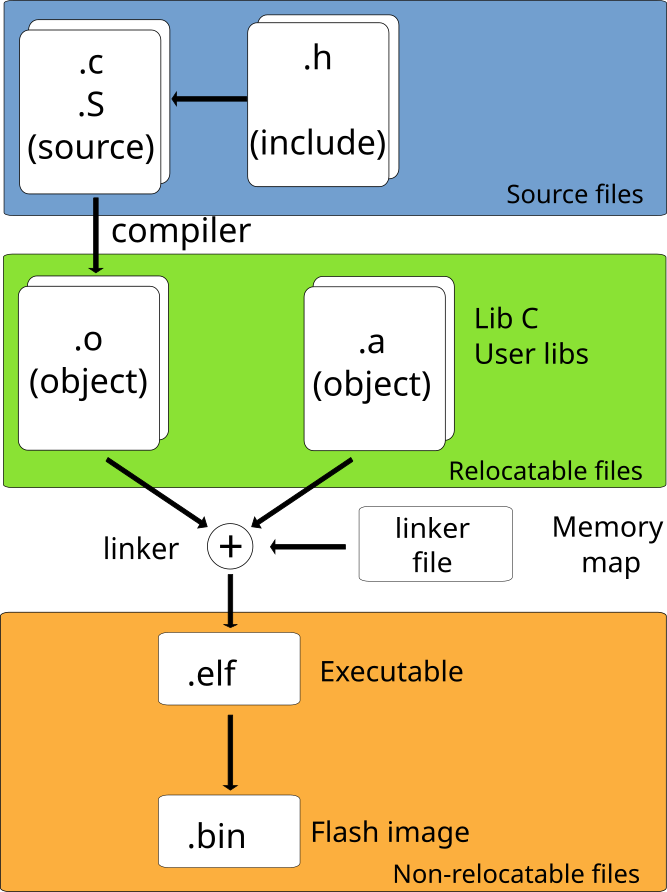
\includegraphics[scale=0.6]{imgs/compile_process.png}
	\end{center}	
\end{frame}

\begin{frame}
	\frametitle{Arquivos de inclusão}
	\begin{columns}[T] % align columns
		\begin{column}{.60\textwidth}
			\lstinputlisting[style=customc]{code/demo.h}
		\end{column}%
		\hfill%
		\begin{column}{.40\textwidth}
			\begin{itemize}
				\item Pense como API: só exporte interfaces e o que elas precisarem !
				\item Não esqueça a proteção de inclusão recursiva !				
				\item Não é ANSI-C mas \texttt{\textcolor{blue}{\#pragma once}} pode ser interessante
				\item Evite incluir arquivos de inclusão como boa prática
			\end{itemize}
		\end{column}%
	\end{columns}
\end{frame}

\begin{frame}
	\frametitle{Arquivos de inclusão}
	\lstinputlisting[style=customc]{code/accel.h}
\end{frame}

\begin{frame}
	\frametitle{Especificadores de classe de armazenamento}
	\begin{center}
		\texttt{\textcolor{blue}{static extern auto register}}
	\end{center}
	\begin{itemize}
		\vspace*{0.5cm}
	\item Uma das características pouco entendidas da linguagem C e frequentemente mal empregadas.
	\item Permitem detalhar a declaração de uma variável, com relação a linkagem, localização, escopo e valores iniciais.
	\item É confuso pois o significado pode mudar de acordo com a posição no código fonte.
	\item Mas, precisamos entender antes como as variáveis são armazenadas !
	\end{itemize}
\end{frame}

\begin{frame}
	\frametitle{Stack (Pilha)}
	\begin{itemize}
		\item Geralmente usado para alocação de variáveis temporárias ou passagem de parâmetros.
		\item É uma região linear de memória, gerida por um registro denominado de \textit{Stack Pointer}.
		\item O compilador analisa o código e gerar instruções para uso do stack.
	\end{itemize}	
\end{frame}

\begin{frame}
	\frametitle{Stack (Pilha)}
	\begin{columns}[T] % align columns
	\begin{column}{.60\textwidth}
		\lstinputlisting[style=customc]{code/stack.c}
	\end{column}%
	\hfill%
	\begin{column}{.40\textwidth}
		Análise:
	\end{column}%
\end{columns}	
\end{frame}

\begin{frame}
	\frametitle{Cuidados no uso da pilha}
	\begin{itemize}
	\item Tamanho de variáveis e estouro de pilha
	\item Recursão ou longo encadeamento de chamadas
	\item Retorno de valores locais
	\item Dimensionamento da pilha
	\end{itemize}	
\end{frame}

\begin{frame}
	\frametitle{Uso de static em variáveis locais}
	\begin{itemize}
	\item Escopo local (não visível fora da função)
	\item Armazenamento em área global (não usa pilha)
	\item Permite valores de inicialização.
	\end{itemize}	
\end{frame}

\begin{frame}
	\frametitle{Stack (Pilha)}
	\begin{columns}[T] % align columns
		\begin{column}{.60\textwidth}
			\lstinputlisting[style=customc]{code/static_var_fun.c}
		\end{column}%
		\hfill%
		\begin{column}{.40\textwidth}
			Análise:
		\end{column}%
	\end{columns}	
\end{frame}

\begin{frame}
	\frametitle{Retorno de valores locais, da pilha, pode ?}
	\begin{center}
	\lstinputlisting[style=customc]{code/stack_ret_a.c}
	\end{center}	
	\pause
	\begin{tikzpicture}[remember picture, overlay]
		\node [xshift=-2cm,yshift=-4cm] at (current page.north east)	{
\includegraphics[scale=0.6]{imgs/ok.png}};
		\node [xshift=-2cm,yshift=-6cm] at (current page.north east)	{
\includegraphics[scale=0.6]{imgs/ok.png}};
		\node [xshift=-2cm,yshift=-8cm] at (current page.north east)	{
\includegraphics[scale=0.6]{imgs/maybe.png}};
	\end{tikzpicture}
\end{frame}

\begin{frame}
	\frametitle{Retorno de valores locais, da pilha, pode ?}
	\begin{center}
		\lstinputlisting[style=customc]{code/stack_ret_b.c}
	\end{center}	
	\pause
	\begin{tikzpicture}[remember picture, overlay]
		\node [xshift=-2cm,yshift=-4cm] at (current page.north east)	{
\includegraphics[scale=0.6]{imgs/maybe.png}};
		\node [xshift=-2cm,yshift=-6cm] at (current page.north east)	{
\includegraphics[scale=0.6]{imgs/nok.png}};
		\node [xshift=-2cm,yshift=-8cm] at (current page.north east)	{
\includegraphics[scale=0.6]{imgs/ok.png}};
\end{tikzpicture}
\end{frame}

\begin{frame}
	\frametitle{Passagem por valor x passagem por referência}
	\begin{itemize}
		\item Passagem por valor: o valor original é copiado e não pode ser alterado pela função
		\item Passagem por referência: 
		\begin{itemize}
			\item O valor original não é copiado e pode ser alterado pela função. É utilizado um ponteiro para essa operação.
			\item Também é interessante quando se passam estruturas muito grandes, economizando memória e processamento
		\end{itemize}
	\end{itemize}
\end{frame}

\begin{frame}[fragile]
	\frametitle{Ponteiros}
	\begin{itemize}
		\item Um ponteiro armazena um valor e não um valor !
		\item São referências indiretas para outras variáveis ou funções
		\item São declarados com o emprego do asterisco \texttt{\textcolor{blue}{``*''}}
		\item Endereços podem ser obtidos com o uso do operador \texttt{\textcolor{blue}{``\&''}}
		\item Declaração básica de variável ponteiro:
	\end{itemize}
	\begin{verbatim}
        <tipo_de_dado> *variavel;
        uint8_t *pbuffer;
        struct accel_s *paccel;
	\end{verbatim}	
\end{frame}

\begin{frame}[fragile]
	\frametitle{Ponteiros para variáveis simples}
	\begin{columns}[T] % align columns
	\begin{column}{.50\textwidth}
		\lstinputlisting[style=customc]{code/ptr_a.c}
	\end{column}%
	\hfill%
	\begin{column}{.50\textwidth}
	 {\tiny 
	\begin{verbatim}
              Memory (32 bits)
           +-------------------+
0x20000000 |      var (10)     |<---+
           +-------------------+    |
0x20000004 |        ...        |    |
           +-------------------+    |
0x20000008 | pvar (0x20000000) |----+
           +-------------------+
0x2000000C |                   |
           +-------------------+
0x20000010 |                   |
           +------------------+
	\end{verbatim}
}

	\end{column}%
\end{columns}	
\end{frame}

\begin{frame}[fragile]
	\frametitle{Ponteiros para estruturas simples}
	\begin{columns}[T] % align columns
	\begin{column}{.75\textwidth}
		\lstinputlisting[style=customc]{code/ptr_b.c}
	\end{column}%
	\hfill%
	\begin{column}{.25\textwidth}
	\end{column}%
\end{columns}	
\end{frame}

\begin{frame}
	\frametitle{Formas de dimensionamento da pilha}
	\begin{itemize}
		\item Análises estáticas
		\begin{itemize}
			\item Usando o próprio compilador (\texttt{-fstack-usage} e \texttt{-fcallgraph-info} no GCC) e analisando o uso da pilha a partir do \texttt{main()} (análise estática)
			\item Usando ferramentas (PC-Lint, valgrind, cppcheck)
			\item Problemas: podem falhar em casos de recursão, interrupções, chamadas indiretas (ponteiros para função)
		\end{itemize}
		\item Análises dinâmicas: técnica da marca d'agua na região do stack (verificação dinâmica, útil em caso de recursão, interrupção)
		\end{itemize}		
\end{frame}

\begin{frame}
	\frametitle{Especificadores de classe de armazenamento (auto)}
\begin{columns}[T] % align columns
	\begin{column}{.60\textwidth}
		\lstinputlisting[style=customc]{code/auto.c}
	\end{column}%
	\hfill%
	\begin{column}{.40\textwidth}
		\begin{center}
			\texttt{\textcolor{blue}{auto}}
		\end{center}
		\vspace*{0.5cm}
		\begin{itemize}
			\item É a classe padrão, de escopo local, armazenadas na RAM (pilha), valor inicial pode ser lixo.
			\item Pode ser omitida, por simplicidade.
		\end{itemize}
	\end{column}%
\end{columns}
\end{frame}

\begin{frame}
	\frametitle{Especificadores de classe de armazenamento}
		\begin{center}
		\texttt{\textcolor{blue}{static}}
		\end{center}
		\vspace*{0.5cm}
		\begin{itemize}
			\item Se usada com variáveis dentro de funções: gera variáveis que mantem valores entre chamadas e são alocadas na área de variáveis globais. São inicializadas com zero, caso não explicitamente especificado.
			\item Se usada com variáveis no escopo do arquivo (fora das funções) o comportamento é o mesmo mas existem diferenças em relação a sua visibilidade.
			\item \texttt{static} também pode ser usada em declarações de função. Novamente, implica em mudança de visibilidade.
			\item Novo conceito requerido: \textbf{linkagem padrão da linguagem C} !
		\end{itemize}
\end{frame}

\begin{frame}
	\frametitle{Especificadores de classe de armazenamento (extern)}
	\begin{columns}[T] % align columns
		\begin{column}{.57\textwidth}
			\lstinputlisting[style=customc]{code/static_linkage_b.c}
			\lstinputlisting[style=customc]{code/static_linkage_a.c}			
		\end{column}%
		\hfill%
		\begin{column}{.43\textwidth}
			\begin{itemize}
				\item Por default, o compilador C externa todos os símbolos gerados (main,var).
				\item Com \texttt{extern}, você pode explicitamente dizer que existe algo externo ao seu arquivo (file2.c) e que pretende usar.
			\item No entanto, mesmo que não especifique nada, o linker vai tentar encontrar algo na tabela de símbolos que resolva a referência.
			\end{itemize}
		\end{column}%
	\end{columns}	
\end{frame}

\begin{frame}
	\frametitle{Especificadores de classe de armazenamento (static/extern)}
	\begin{columns}[T] % align columns
		\begin{column}{.57\textwidth}
			\lstinputlisting[style=customc]{code/static_linkage_e.c}			
			\lstinputlisting[style=customc]{code/static_linkage_d.c}
			\lstinputlisting[style=customc]{code/static_linkage_c.c}
		\end{column}%
		\hfill%
		\begin{column}{.43\textwidth}
			\begin{itemize}
				\item Agora \texttt{var} tem \textbf{linkagem interna}, não é mais vista fora de file2.c (o símbolo não é exportado)
				\item Conceito também válido para funções \texttt{static} !
				\item Princípio de encapsulamento ou API.
			\end{itemize}
		\end{column}%
	\end{columns}	
\end{frame}

\begin{frame}
	\frametitle{Especificadores de classe de armazenamento}
	\begin{center}
		\texttt{\textcolor{blue}{register}}
	\end{center}
	\vspace*{0.5cm}
	\begin{itemize}
		\item Se usada com variáveis dentro de funções.
		\item Indica ao compilador que deseja o armazenamento da variável em um registro do processador (geralmente para maior performance).
		\item Pouco útil atualmente, em geral o compilador resolve bem essas situações.
	\end{itemize}
\end{frame}

\begin{frame}
	\frametitle{Arquivos de código fonte}
	\begin{columns}[T] % align columns
		\begin{column}{.60\textwidth}
			\lstinputlisting[style=customc]{code/demo.c}
		\end{column}%
		\hfill%
		\begin{column}{.40\textwidth}
			\begin{itemize}
				\item Externe via funções o acesso a seus dados internos (encapsulamento)
				\item Dê escopo de arquivo para as suas funções e variáveis com \texttt{static} !
				\item Salve RAM colocando como \texttt{const} o que for realmente constante.
			\end{itemize}
		\end{column}%
	\end{columns}
\end{frame}

\begin{frame}
	\frametitle{Arquivos de código fonte}
	\lstinputlisting[style=customc]{code/accel.c}
\end{frame}


\begin{frame}[fragile]
	\begin{lstlisting}[style=customc]
		// test
		#include <stdio.h>
		int main(void)
		{
			printf("Hello World!"); 
		}
	\end{lstlisting}
\end{frame}

\begin{frame}
	\frametitle{Palavras Reservadas}
	\begin{itemize}
		\item x
	\end{itemize}	
\end{frame}

\begin{frame}
	\frametitle{}
	\begin{columns}[T] % align columns
		\begin{column}{.50\textwidth}
		\end{column}%
		\hfill%
		\begin{column}{.50\textwidth}
		\end{column}%
	\end{columns}
\end{frame}

\end{document}


% https://aticleworld.com/dangling-pointer-and-memory-leak/
% const em ponteiros